\documentclass[11pt]{article}
\usepackage{amsmath, amssymb, graphicx, hyperref, natbib}
\usepackage[margin=1in]{geometry}
\usepackage{tikz}
\usepackage{pgfplots}
\usetikzlibrary{3d, positioning, arrows.meta, calc}
\title{Iterated Closest Point (ICP) for Scan Matching in SLAM Applications}
\author{Oliver MacDonald}
\date{\today}

\begin{document}
\maketitle

\begin{abstract}
This paper investigates the mathematical foundations, implementation, and evaluation of Iterative Closest Point (ICP) algorithms for scan matching, a core component of SLAM (Simultaneous Localization and Mapping) in autonomous robotic systems. Variants including point-to-point, point-to-plane, and Generalized ICP are examined with respect to accuracy, convergence, and computational cost in the context of edge device deployment for lunar robotics.
\end{abstract}

\section{Introduction}

Autonomous navigation has become a major focus of modern robotics, especially in environments where external positioning systems like GPS are unavailable. This challenge is emphasized by the NASA Lunabotics competition, in which Boise State University's Bender Robotics Team is competing with their fully autonomous lunar excavation robot, \textit{Bender}. The robot is tasked with navigating rough, dusty terrain, collecting regolith, and returning it to a specified location—entirely without human intervention.

% Include photo of Bender Lunabotics Edition

Bender employs a multi-sensor architecture that includes 3D LiDAR, stereo cameras, an IMU, and a Vive beacon system for indoor positional tracking. Despite this advanced suite, the navigation stack has exhibited failure modes, particularly in odometry and mapping. These failures manifest as “tornado mode,” in which accumulated error causes the map to rotate around the robot, resulting in incorrect obstacle detection and incorrect positioning. This ultimately forces the robot to make incorrect navigation decisions, such as turning in place indefinitely or abandoning its planned path.

% Include photo of Bender 3.14 when in tornado mode

In GPS-denied environments like the lunar surface, correcting this drift without an external reference requires accurate scan matching between consecutive LiDAR frames. Iterative Closest Point (ICP) algorithms offer a compelling solution, using geometric relationships between overlapping point clouds to estimate the robot's motion and update the map. However, ICP comes with trade-offs between computational cost and alignment accuracy, which are especially relevant for embedded platforms like the ESP32, Teensy 4.1, and Raspberry Pi 5, where real-time constraints demand <10ms compute cycles.

The objective of this work is to analyze and compare three major variants of the ICP algorithm being Point-to-Point, Point-to-Plane, and Generalized ICP. This paper focuses on their mathematical formulation, numerical stability, and suitability for real-time implementation on constrained hardware. The aim is to determine which variant provides the best balance of performance and computational cost for potential deployment on the Bender robot during the final testing phase.

The project contribution is twofold:
\begin{itemize}
    \item A structured evaluation of ICP variants using both Python prototypes and C-based embedded implementations.
    \item A set of recommendations for deploying accurate, lightweight scan matching algorithms for real-time SLAM on edge robotics platforms.
\end{itemize}

\section{ICP Algorithm Variants}

\subsection{Point-to-Point ICP}
Point-to-point ICP seeks the transformation $T = (R, \mathbf{t})$ that minimizes the sum of squared Euclidean distances between corresponding points in the source and target point clouds:
\[
E(R, \mathbf{t}) = \sum_{i=1}^N \| \mathbf{q}_i - (R\mathbf{p}_i + \mathbf{t}) \|^2
\]
This approach assumes that all point correspondences are valid and carries the risk of local minima when the overlap is poor. The optimal transformation is solved via SVD on the cross-covariance matrix between centered point clouds \citep{donoso2017icp}.

\begin{figure}[h]
\centering
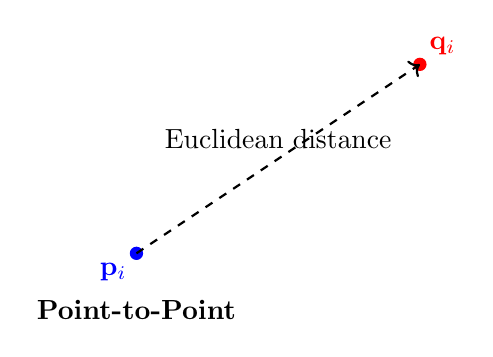
\begin{tikzpicture}[scale=1.2]
  % Source and target points
  \fill[blue] (0,0) circle (2pt) node[below left] {$\mathbf{p}_i$};
  \fill[red] (3,2) circle (2pt) node[above right] {$\mathbf{q}_i$};

  % Arrow showing Euclidean match
  \draw[->, thick, dashed] (0,0) -- (3,2) node[midway, above] {Euclidean distance};

  % Origin
  \node at (0,-0.6) {\textbf{Point-to-Point}};
\end{tikzpicture}
\caption{Point-to-Point ICP minimizes direct Euclidean distance between corresponding points.}
\label{fig:ptp_icp}
\end{figure}  

\subsection{Point-to-Plane ICP}
Point-to-plane ICP leverages local surface normals to minimize the distance from each source point to the tangent plane at the corresponding target point. The objective function becomes:
\[
E(R, \mathbf{t}) = \sum_{i=1}^N \left[ \mathbf{n}_i^\top (\mathbf{q}_i - (R\mathbf{p}_i + \mathbf{t})) \right]^2
\]
This leads to a linear least squares system solved via QR decomposition. It tends to converge faster than point-to-point ICP, especially when surface geometry is well-defined \citep{guevara2024scan}.

\begin{figure}[h]
\centering
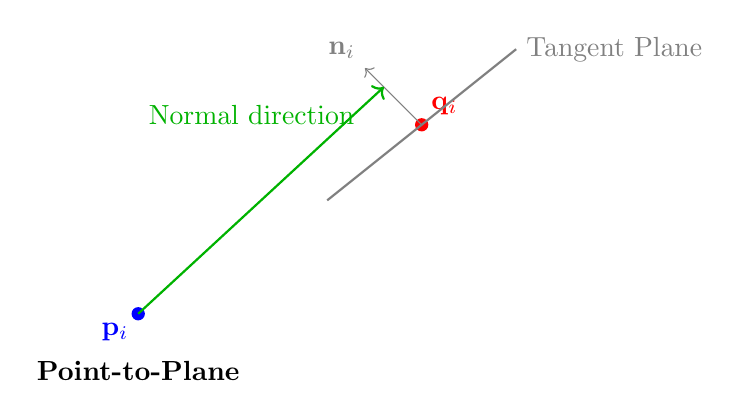
\begin{tikzpicture}[scale=1.2]
  % Source point
  \fill[blue] (0,0) circle (2pt) node[below left] {$\mathbf{p}_i$};

  % Target point
  \fill[red] (3,2) circle (2pt) node[above right] {$\mathbf{q}_i$};

  % Plane line (normal)
  \draw[gray, thick] (2,1.2) -- (4,2.8) node[gray,right] {Tangent Plane};

  % Normal vector at q_i
  \draw[->, gray] (3,2) -- ++(-0.6,0.6) node[above left] {$\mathbf{n}_i$};

  % Projection from p_i to plane
  \draw[->, thick, green!70!black] (0,0) -- (2.6,2.4);
  \node[green!70!black] at (1.2,2.1) {Normal direction};

  \node at (0,-0.6) {\textbf{Point-to-Plane}};
\end{tikzpicture}
\caption{Point-to-Plane ICP minimizes distance along the normal vector of the target surface.}
\label{fig:ptpl_icp}
\end{figure}  

\subsection{Generalized ICP}
Generalized ICP (G-ICP) fuses point-to-point and point-to-plane ideas into a probabilistic framework. Each point is modeled as a Gaussian with associated covariance:
\[
E(T) = \sum_{i=1}^N (\mathbf{q}_i - T\mathbf{p}_i)^\top (C_q + R C_p R^\top)^{-1} (\mathbf{q}_i - T\mathbf{p}_i)
\]
This formulation improves robustness to noise and outliers by weighting residuals based on local uncertainty. It reduces sensitivity to poor correspondences and unifies multiple ICP variants under a common model \citep{segal2009gicp}.

\begin{figure}[h]
\centering
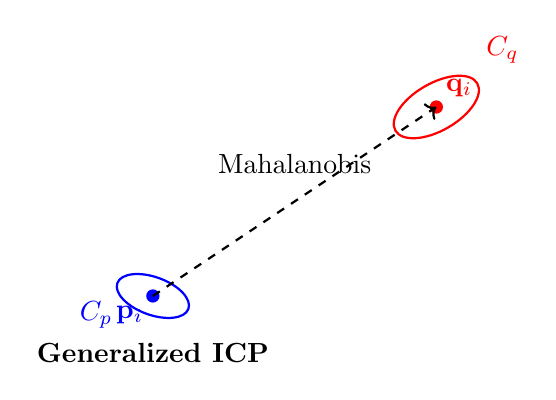
\begin{tikzpicture}[scale=1.2]
  % Source point
  \fill[blue] (0,0) circle (2pt) node[below left] {$\mathbf{p}_i$};
  \draw[blue, thick, rotate around={-20:(0,0)}] (0,0) ellipse (0.4 and 0.2);
  \node[blue] at (-0.6,-0.2) {$C_p$};

  % Target point
  \fill[red] (3,2) circle (2pt) node[above right] {$\mathbf{q}_i$};
  \draw[red, thick, rotate around={30:(3,2)}] (3,2) ellipse (0.5 and 0.25);
  \node[red] at (3.7,2.6) {$C_q$};

  % Match line
  \draw[->, thick, dashed] (0,0) -- (3,2);
  \node at (1.5,1.4) {Mahalanobis};

  \node at (0,-0.6) {\textbf{Generalized ICP}};
\end{tikzpicture}
\caption{G-ICP minimizes Mahalanobis distance using local point covariances.}
\label{fig:gicp}
\end{figure}  

\subsection{Comparison Framework}
To assess the practical trade-offs of ICP variants, we compare them using:

\begin{itemize}
  \item \textbf{Metrics}: Accuracy (final alignment error), Precision (variance over trials), and Runtime (ms/frame)
  \item \textbf{Datasets}: Both synthetic point clouds (e.g., shapes, noisy transforms) and real-world terrain data
  \item \textbf{Target Platforms}: Raspberry Pi 5, Teensy 4.1, and ESP32 for embedded deployment constraints
\end{itemize}

\section{Formulation}
\subsection{Rigid Transformations in 3D}

A rigid body transformation $T$ in 3D applies a rotation $R \in SO(3)$ and translation $\mathbf{t} \in \mathbb{R}^3$ to a point $\mathbf{p} \in \mathbb{R}^3$:
\[
T(\mathbf{p}) = R\mathbf{p} + \mathbf{t}
\]

\begin{figure}[h]
\centering
\begin{tikzpicture}[scale=1.0]
  % Axes
  \draw[->] (0,0) -- (3,0) node[right] {$x$};
  \draw[->] (0,0) -- (0,3) node[above] {$y$};
  \draw[->] (0,0) -- (1.5,-1.5) node[below] {$z$};

  % Original point
  \fill[blue] (1,1) circle (2pt) node[above left] {$\mathbf{p}$};

  % Transformed point
  \fill[red] (2.5,2.2) circle (2pt) node[above right] {$T(\mathbf{p})$};
  \draw[->, dashed] (1,1) -- (2.5,2.2) node[midway, above] {$R, \mathbf{t}$};

  % Origin label
  \node[below left] at (0,0) {O};
\end{tikzpicture}
\caption{Rigid transformation in 3D showing rotation $R$ and translation $\mathbf{t}$.}
\end{figure}

Rigid transformations preserve distances and angles, which is crucial for physical scan alignment tasks.

\subsection{Point Cloud Registration}

Given a source point cloud $\mathcal{P} = \{\mathbf{p}_i\}$ and a target (map) point cloud $\mathcal{Q} = \{\mathbf{q}_i\}$, ICP attempts to find the transformation $T = (R, \mathbf{t})$ that minimizes alignment error:
\[
T^* = \arg\min_{R, \mathbf{t}} \sum_i \| \mathbf{q}_i - (R\mathbf{p}_i + \mathbf{t}) \|^2
\]
This assumes point correspondences $(\mathbf{p}_i, \mathbf{q}_i)$ are known or estimated via nearest neighbor search. Variants modify the error metric, correspondence criteria, and optimization strategy.

\subsection{Least Squares \& SVD for Best-Fit Transform}

For point-to-point ICP, once correspondences are determined, we solve for $T^*$ by minimizing the Frobenius norm of residuals. Centering both point sets (by subtracting their means) leads to an orthogonal Procrustes problem:
\[
\min_R \| R\mathbf{P}_c - \mathbf{Q}_c \|_F^2
\]
This is solved using Singular Value Decomposition (SVD) on the cross-covariance matrix $H = \sum_i \mathbf{p}_i \mathbf{q}_i^\top$. Let $H = U\Sigma V^\top$, then $R = VU^\top$ ensures the closest orthogonal matrix through a least squares approach.

\subsection{Overdetermined Systems \& QR Decomposition}

For point-to-plane ICP, we minimize the orthogonal distance from a transformed point to the tangent plane of its correspondence:
\[
E = \sum_i \left[ \mathbf{n}_i^\top (\mathbf{q}_i - R\mathbf{p}_i - \mathbf{t}) \right]^2
\]
This is linearized using small-angle approximations and solved via the least squares method:
\[
Ax = b \quad \text{where} \quad A \in \mathbb{R}^{N \times 6},\; x = [\delta \theta_x, \delta \theta_y, \delta \theta_z, t_x, t_y, t_z]^\top
\]
The overdetermined system is efficiently solved with QR decomposition or normal equations.

\subsection{Covariance \& Probabilistic Models in G-ICP}

In Generalized ICP, each point in the source and target cloud is treated as a Gaussian-distributed random variable:
\[
\mathbf{p}_i \sim \mathcal{N}(\hat{\mathbf{p}}_i, C_p), \quad \mathbf{q}_i \sim \mathcal{N}(\hat{\mathbf{q}}_i, C_q)
\]

The goal is to minimize the Mahalanobis distance between transformed source points and their targets:
\[
T^* = \arg\min_T \sum_i (\mathbf{q}_i - T\mathbf{p}_i)^\top (C_q + R C_p R^\top)^{-1} (\mathbf{q}_i - T\mathbf{p}_i)
\]

The covariance matrices $C_p$ and $C_q$ describe local surface uncertainty, estimated via PCA in a local neighborhood.

\begin{figure}[h]
\centering
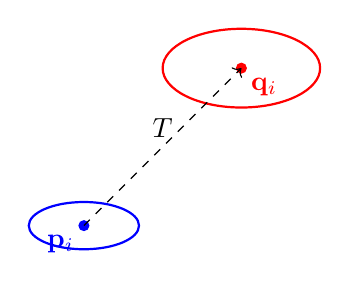
\begin{tikzpicture}[scale=1.0]
  % Target ellipse
  \draw[red, thick] (2,2) ellipse (1 and 0.5);
  \fill[red] (2,2) circle (2pt) node[below right] {$\mathbf{q}_i$};

  % Source ellipse
  \draw[blue, thick] (0,0) ellipse (0.7 and 0.3);
  \fill[blue] (0,0) circle (2pt) node[below left] {$\mathbf{p}_i$};

  % Arrow showing transformation
  \draw[->, dashed] (0,0) -- (2,2) node[midway, above] {$T$};
\end{tikzpicture}
\caption{Covariance ellipses for a source-target pair in G-ICP. Uncertainty is modeled via local PCA.}
\end{figure}

Unlike standard ICP, G-ICP weighs the alignment based on both structural orientation and measurement noise, resulting in a more robust and symmetric scan matching framework \citep{segal2009gicp}.

\section{Implementation}

Both Python and C++ versions were created to support rapid development, benchmarking, and eventual deployment on embedded hardware platforms. The framework supports Point-to-Point, Point-to-Plane, and Generalized ICP variants.

\subsection{Python Implementation Overview}

The Python implementation is designed for modularity and experimentation. A central \texttt{icp.py} module defines a base \texttt{ICPAlgorithm} class, which is subclassed by \texttt{PointToPointICP}, \texttt{PointToPlaneICP}, and \texttt{GeneralizedICP}. Each variant follows a consistent API, supporting plug-and-play benchmarking across different datasets.

Point correspondence is handled using multiple nearest neighbor strategies implemented via \texttt{scikit-learn}'s \texttt{NearestNeighbors}. Local normals and covariances are estimated using PCA on k-NN neighborhoods. Visualization is performed using \texttt{matplotlib} for 2D cases and \texttt{plotly} for 3D scenes.

Configurations for each run are specified using a custom \texttt{ICPConfig} data class:
\begin{itemize}
    \item \textbf{Segmentation}: \texttt{none}, \texttt{even\_points}, \texttt{even\_range}, \texttt{uneven\_points}
    \item \textbf{Filtering}: Dropout percentage via Gaussian noise filtering
    \item \textbf{Memory Modes}: \texttt{full}, \texttt{previous}, \texttt{sliding} (controls map history size)
    \item \textbf{Rejection Criteria}: Max distance, normal difference threshold, percentile clipping
    \item \textbf{Neighborhood Search}: \texttt{fixed} radius or \texttt{density\_adaptive}
    \item \textbf{Optional}: Number of map segments, density factors
\end{itemize}

This structure enables reproducible experimentation and makes it easy to test new matching, filtering, or segmentation strategies.

\subsection{C/PlatformIO Version Overview}

The C++ implementation is designed for deployment on embedded systems and is integrated into a larger SLAM system currently under development. It uses the PlatformIO build system to target both the Teensy 4.1 and ESP32 microcontrollers.

All three ICP variants are implemented in C++ using the \texttt{Eigen} linear algebra library to support efficient matrix and vector operations. The ICP module is class-based and can be compiled independently or linked into larger robotic frameworks. The system is compatible with fixed-point math and optimized for deterministic behavior under low-power, real-time constraints.

\subsection{Edge Deployment Strategy}

The ultimate goal of this work is to identify which ICP variant best balances runtime and accuracy on constrained hardware. For this reason, the system is designed to operate within a strict \textless10\,ms processing window per frame.

Before scan matching, all sensor data (LiDAR, IMU, etc.) is merged into a shared spatial grid using fixed-point math. This preprocessing ensures that the ICP module operates on a consistent input space. The resulting transformation estimates are streamed via serial to a base station or visualized in real-time for debugging.

Variant selection is currently manual, with this research aimed at recommending the most effective variant for real deployment scenarios.

\subsection{Test Scenarios and Parameters}

Testing is performed using both synthetic datasets and real-world LiDAR scans. Synthetic scans are used to validate correctness under known transformations, while real LiDAR frames simulate practical deployment conditions. Due to ongoing hardware repairs, full system testing with the Bender robot is pending.

Test cases include both translation and rotation, and performance is measured using alignment error and runtime per frame. While comprehensive parameter sweeps and statistical robustness checks are desirable, they are currently limited due to time constraints. However, the system is built to easily support such evaluations in future work.

\section{Results}
\subsection{Accuracy and Drift Over Time}
\subsection{Runtime Performance}
\subsection{Convergence Behavior}
\subsection{Hardware-Specific Observations}

\section{Conclusion}
\begin{itemize}
  \item Summary of findings
  \item Recommended ICP variant for lunar robotics
  \item Future work: robust data association, SLAM loop closure
\end{itemize}

\bibliographystyle{plainnat}
\bibliography{references}

\appendix
\section{Programs Used}
\begin{itemize}
  \item Python: NumPy, SciPy, Open3D
  \item C: Eigen, PlatformIO libraries for Teensy and Raspberry Pi
  \item Visualization: Matplotlib \& Plotly for Python implementation, custom C++ visualization using serial output to python interface
\end{itemize}

\end{document}
